% Options for packages loaded elsewhere
\PassOptionsToPackage{unicode}{hyperref}
\PassOptionsToPackage{hyphens}{url}
\documentclass[
  ignorenonframetext,
]{beamer}
\newif\ifbibliography
\usepackage{pgfpages}
\setbeamertemplate{caption}[numbered]
\setbeamertemplate{caption label separator}{: }
\setbeamercolor{caption name}{fg=normal text.fg}
\beamertemplatenavigationsymbolsempty
% remove section numbering
\setbeamertemplate{part page}{
  \centering
  \begin{beamercolorbox}[sep=16pt,center]{part title}
    \usebeamerfont{part title}\insertpart\par
  \end{beamercolorbox}
}
\setbeamertemplate{section page}{
  \centering
  \begin{beamercolorbox}[sep=12pt,center]{section title}
    \usebeamerfont{section title}\insertsection\par
  \end{beamercolorbox}
}
\setbeamertemplate{subsection page}{
  \centering
  \begin{beamercolorbox}[sep=8pt,center]{subsection title}
    \usebeamerfont{subsection title}\insertsubsection\par
  \end{beamercolorbox}
}
% Prevent slide breaks in the middle of a paragraph
\widowpenalties 1 10000
\raggedbottom
\AtBeginPart{
  \frame{\partpage}
}
\AtBeginSection{
  \ifbibliography
  \else
    \frame{\sectionpage}
  \fi
}
\AtBeginSubsection{
  \frame{\subsectionpage}
}
\usepackage{iftex}
\ifPDFTeX
  \usepackage[T1]{fontenc}
  \usepackage[utf8]{inputenc}
  \usepackage{textcomp} % provide euro and other symbols
\else % if luatex or xetex
  \usepackage{unicode-math} % this also loads fontspec
  \defaultfontfeatures{Scale=MatchLowercase}
  \defaultfontfeatures[\rmfamily]{Ligatures=TeX,Scale=1}
\fi
\usepackage{lmodern}
\ifPDFTeX\else
  % xetex/luatex font selection
\fi
% Use upquote if available, for straight quotes in verbatim environments
\IfFileExists{upquote.sty}{\usepackage{upquote}}{}
\IfFileExists{microtype.sty}{% use microtype if available
  \usepackage[]{microtype}
  \UseMicrotypeSet[protrusion]{basicmath} % disable protrusion for tt fonts
}{}
\makeatletter
\@ifundefined{KOMAClassName}{% if non-KOMA class
  \IfFileExists{parskip.sty}{%
    \usepackage{parskip}
  }{% else
    \setlength{\parindent}{0pt}
    \setlength{\parskip}{6pt plus 2pt minus 1pt}}
}{% if KOMA class
  \KOMAoptions{parskip=half}}
\makeatother
\usepackage{longtable,booktabs,array}
\newcounter{none} % for unnumbered tables
\usepackage{calc} % for calculating minipage widths
\usepackage{caption}
% Make caption package work with longtable
\makeatletter
\def\fnum@table{\tablename~\thetable}
\makeatother
\usepackage{graphicx}
\makeatletter
\newsavebox\pandoc@box
\newcommand*\pandocbounded[1]{% scales image to fit in text height/width
  \sbox\pandoc@box{#1}%
  \Gscale@div\@tempa{\textheight}{\dimexpr\ht\pandoc@box+\dp\pandoc@box\relax}%
  \Gscale@div\@tempb{\linewidth}{\wd\pandoc@box}%
  \ifdim\@tempb\p@<\@tempa\p@\let\@tempa\@tempb\fi% select the smaller of both
  \ifdim\@tempa\p@<\p@\scalebox{\@tempa}{\usebox\pandoc@box}%
  \else\usebox{\pandoc@box}%
  \fi%
}
% Set default figure placement to htbp
\def\fps@figure{htbp}
\makeatother
\setlength{\emergencystretch}{3em} % prevent overfull lines
\providecommand{\tightlist}{%
  \setlength{\itemsep}{0pt}\setlength{\parskip}{0pt}}
\usepackage{bookmark}
\IfFileExists{xurl.sty}{\usepackage{xurl}}{} % add URL line breaks if available
\urlstyle{same}
\hypersetup{
  pdftitle={Categorial Grammar and String Diagrams},
  hidelinks,
  pdfcreator={LaTeX via pandoc}}

\title{\texorpdfstring{Categorial Grammar and String
Diagrams}{Categorial Grammar and String Diagrams}}
\author{\texorpdfstring{}{}}
\date{}

\begin{document}
\frame{\titlepage}

\section{Categorial Grammar, Pregroup Types, and String
Diagrams}\label{sec:categorial-grammar}

\begin{frame}{From Phrase Structure Rules to Algebraic Type Assignment}
\protect\phantomsection\label{from-phrase-structure-rules-to-algebraic-type-assignment}
Traditional generative grammar assigns sentence structure through
phrase-structure rules that recursively combine constituents into larger
units. Categorial grammar inverts this perspective: rather than
specifying construction rules, it assigns each lexical item a
\emph{type} that encodes its combinatory potential. A transitive verb
like ``chases'' is not described as ``a word that takes a subject NP and
an object NP to form a VP'' but rather as having the type
\((n \backslash s) / n\)---an entity that seeks a noun to its right (the
object) and a noun to its left (the subject) in order to produce a
sentence.
\end{frame}

\begin{frame}{Lambek's Residuated Syntactic Calculus}
\protect\phantomsection\label{lambeks-residuated-syntactic-calculus}
The algebraic foundations were laid by Lambek
{[}-@lambek1958mathematics{]}, who introduced a \emph{residuated}
structure on syntactic types: two binary operations, the left residual
\(\backslash\) and the right residual \(/\) of the multiplicative
connective \(\otimes\) (concatenation). The key axiom is the residuation
law:

\[A \otimes B \leq C \quad \iff \quad A \leq C / B \quad \iff \quad B \leq A \backslash C\]

This law captures the fundamental duality of syntax: a verb of type
\((n \backslash s) / n\) \emph{consumes} noun arguments to
\emph{produce} a sentence. The resulting \textbf{Lambek calculus} is a
non-commutative intuitionistic linear logic---non-commutative because
word order matters, and linear because each resource (word) is used
exactly once.

\begin{block}{Pregroup Grammars and Compact Closed Structure}
\protect\phantomsection\label{pregroup-grammars-and-compact-closed-structure}
Lambek {[}-@lambek2004fine{]} later simplified the framework to
\textbf{pregroup grammars}, where each type \(a\) has a left adjoint
\(a^l\) and a right adjoint \(a^r\) satisfying:

\[a^l \cdot a \leq 1 \leq a \cdot a^l \qquad a \cdot a^r \leq 1 \leq a^r \cdot a\]

This formal structuralism was revolutionized by Coecke, Sadrzadeh, and
Clark's introduction of the \textbf{DisCoCat} (Distributional
Compositional Categorical) model in 2010 {[}-@coecke2010mathematical{]}.
DisCoCat unifies categorial grammar with distributional semantics by
defining strong monoidal functors from pregroup grammars to vector
spaces. As Duneau (2021) summarizes, ``The distributional compositional
approach to modelling meaning\ldots{} allows the meaning of a sentence
to be computed as a function of both the distributional meaning of the
words involved, as well as its grammatical form''
{[}-@duneau2021parsing{]}. By demonstrating that pregroups and
finite-dimensional vector spaces are both rigid monoidal categories,
DisCoCat enables sentence meanings to be computed linearly from
constituent word meanings.

Grammaticality reduces to checking whether a sequence of types reduces
to the sentence type \(s\) via these \emph{contraction}
(\(a^l \cdot a \to 1\)) and \emph{expansion} (\(1 \to a \cdot a^l\))
steps. This reformulation is crucial for the DisCoCat framework
(\autoref{sec:categorical-semantics}) because pregroups form
\textbf{compact closed categories}, which have a well-developed
diagrammatic calculus.
\end{block}
\end{frame}

\begin{frame}{String Diagrams for Syntactic Derivation}
\protect\phantomsection\label{string-diagrams-for-syntactic-derivation}
The pivotal connection between categorial grammar and visualization
comes from Joyal and Street {[}-@joyalstreet1991geometry{]}, who proved
that morphisms in monoidal categories can be faithfully represented as
\emph{string diagrams}---planar graphs where:

\begin{itemize}
\tightlist
\item
  \textbf{Wires} represent types (objects of the category)
\item
  \textbf{Boxes} represent words or operations (morphisms)
\item
  \textbf{Vertical composition} represents sequential application
\item
  \textbf{Horizontal juxtaposition} represents the tensor product
  (concatenation)
\item
  \textbf{Cups and caps} represent the contraction/expansion of a
  pregroup
\end{itemize}

\autoref{fig:string-diagram} shows a DisCoCat-style string diagram for
the sentence ``Alice chases Bob,'' generated by our visualization
pipeline. The noun wires connect to the verb's input slots, and the
sentence wire emerges from the verb's output---the entire derivation
from word types to sentence type is visible at a glance.

\begin{figure}
\centering
\pandocbounded{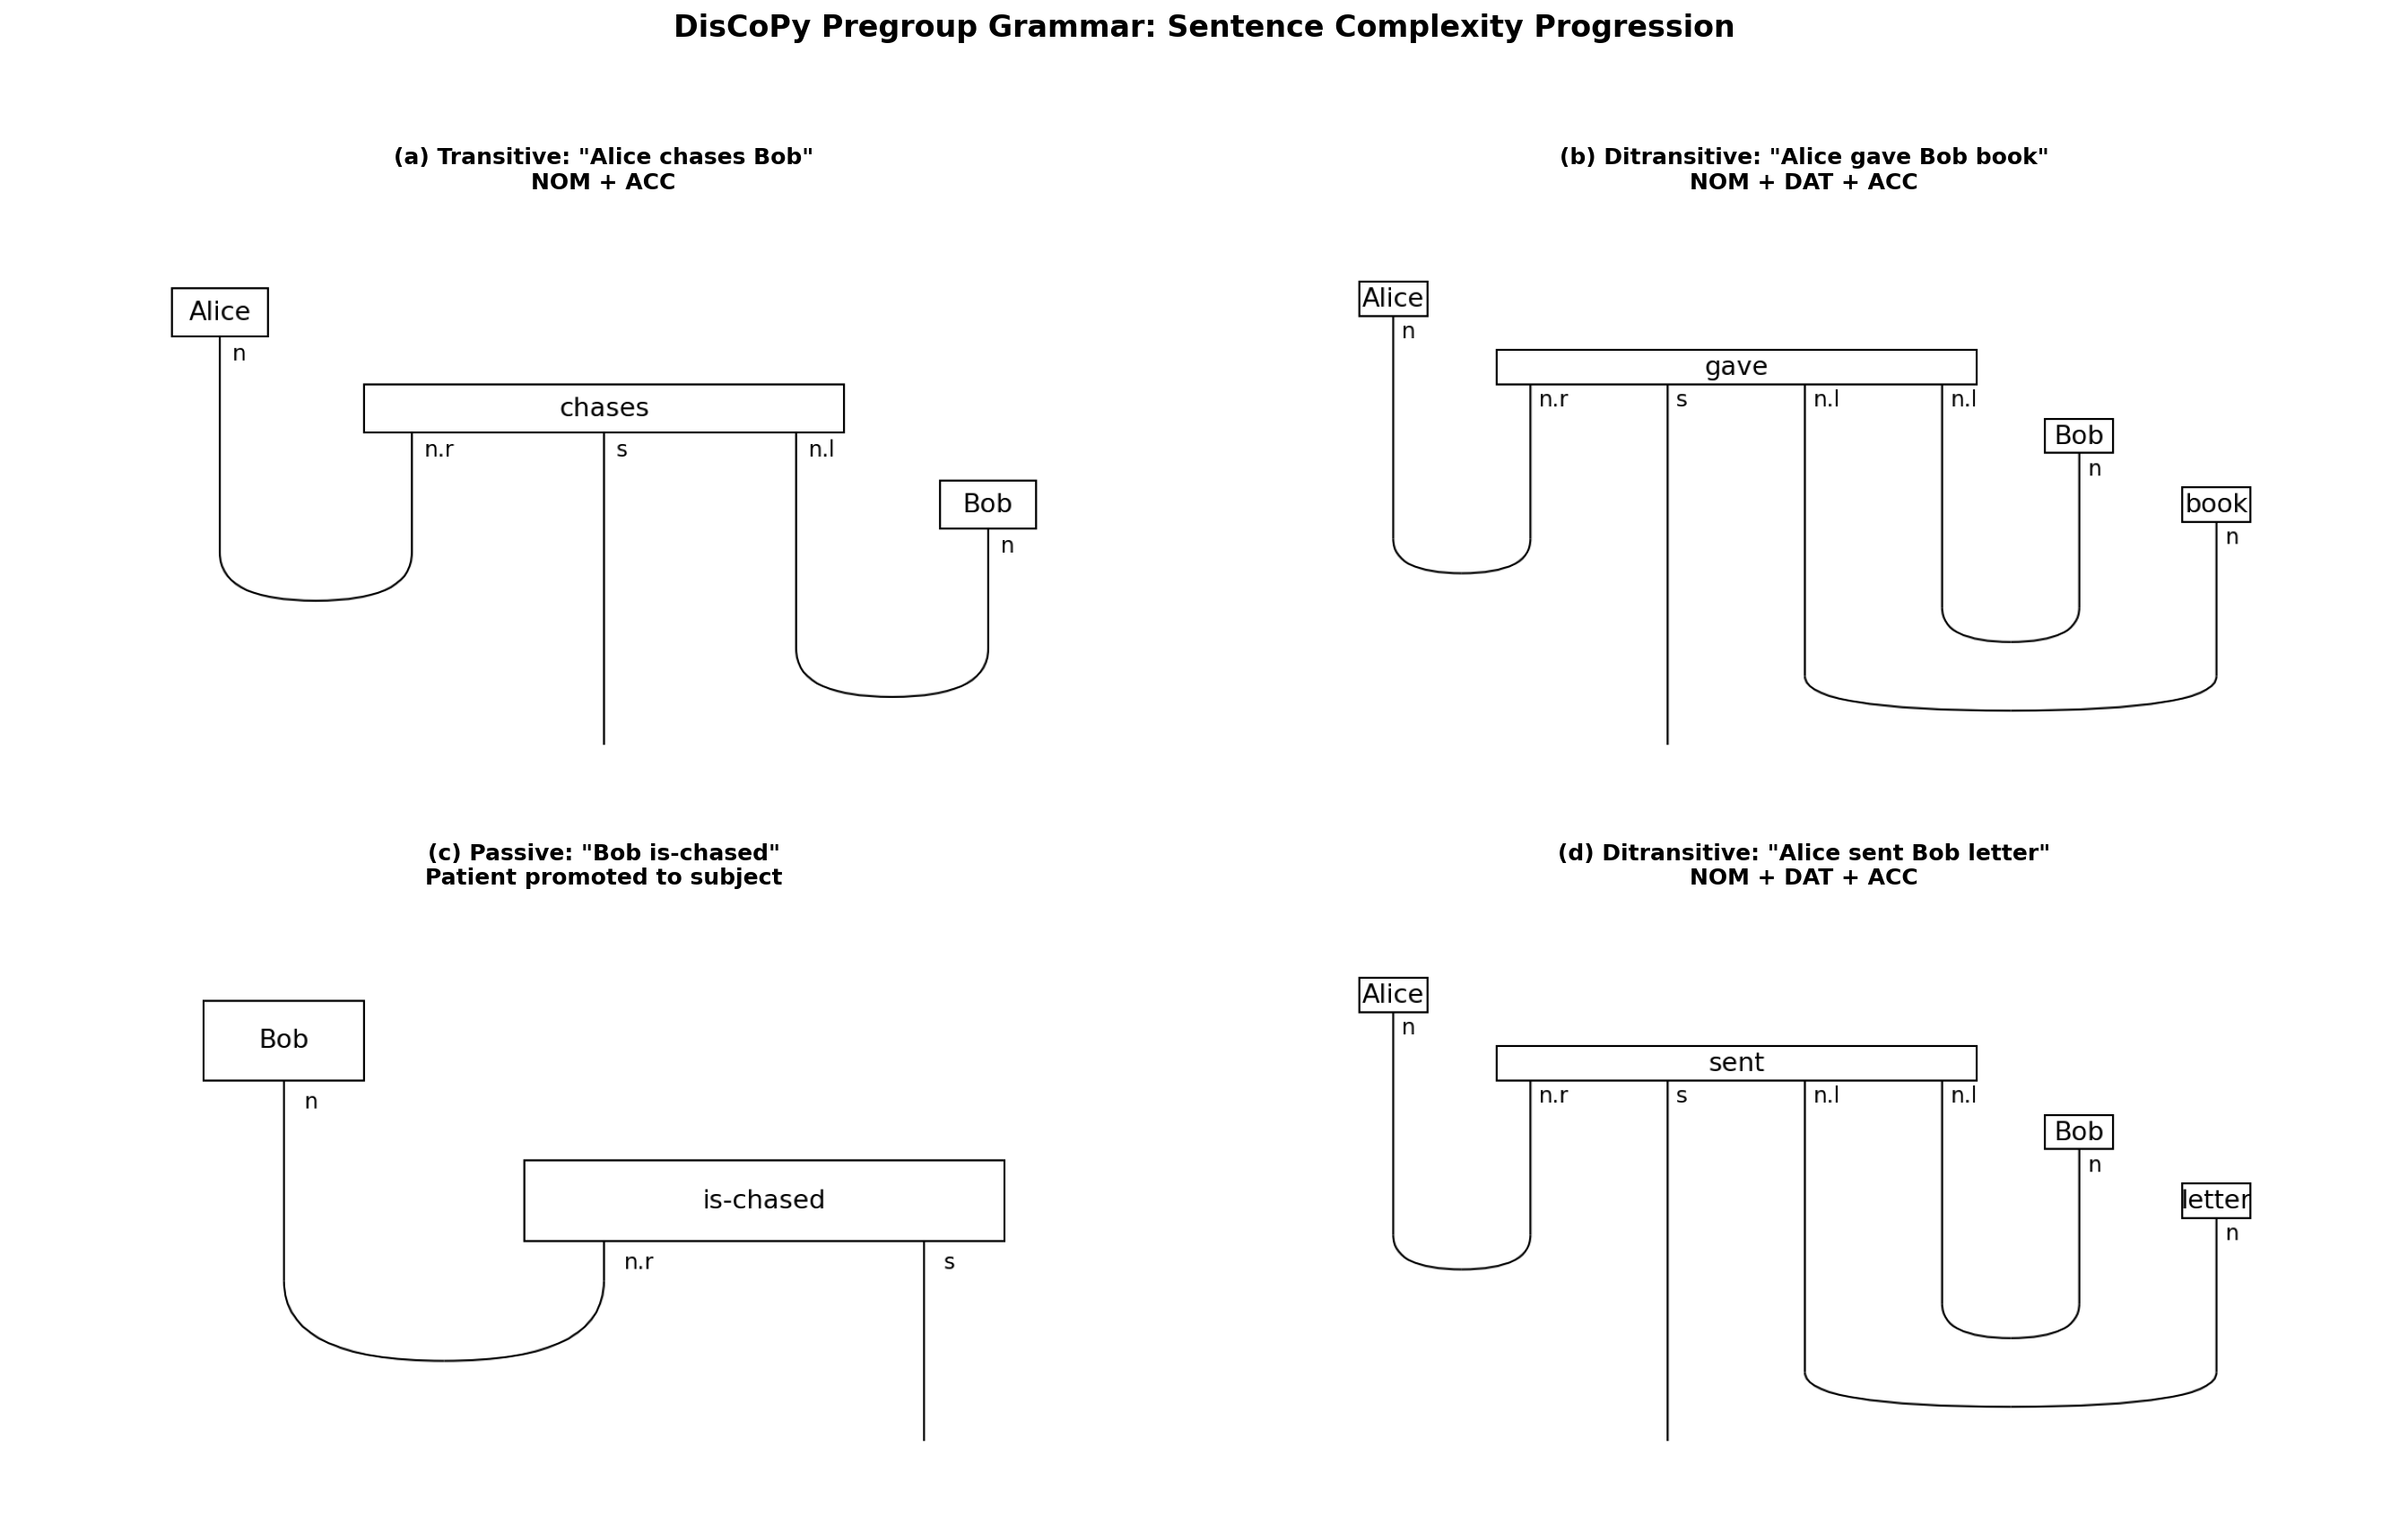
\includegraphics[keepaspectratio,alt={A 2×2 grid of DisCoPy pregroup grammar derivations showing increasing sentence complexity. Panel (a): transitive ``Alice chases Bob'' (NOM+ACC) with two cups contracting noun types into the verb. Panel (b): ditransitive ``Alice gave Bob book'' (NOM+DAT+ACC) with three cups and cascading contractions. Panel (c): passive ``Bob is-chased'' showing patient promotion to subject position via a reduced pregroup type. Panel (d): ditransitive variant ``Alice sent Bob letter'' demonstrating the same NOM+DAT+ACC pattern with different lexical items, confirming structural regularity across verbs.}]{../figures/discopy_sentence_progression.png}}
\caption{A 2×2 grid of DisCoPy pregroup grammar derivations showing
increasing sentence complexity. Panel (a): transitive ``Alice chases
Bob'' (NOM+ACC) with two cups contracting noun types into the verb.
Panel (b): ditransitive ``Alice gave Bob book'' (NOM+DAT+ACC) with three
cups and cascading contractions. Panel (c): passive ``Bob is-chased''
showing patient promotion to subject position via a reduced pregroup
type. Panel (d): ditransitive variant ``Alice sent Bob letter''
demonstrating the same NOM+DAT+ACC pattern with different lexical items,
confirming structural regularity across
verbs.}\label{fig:string-diagram}
\end{figure}

\begin{figure}
\centering
\pandocbounded{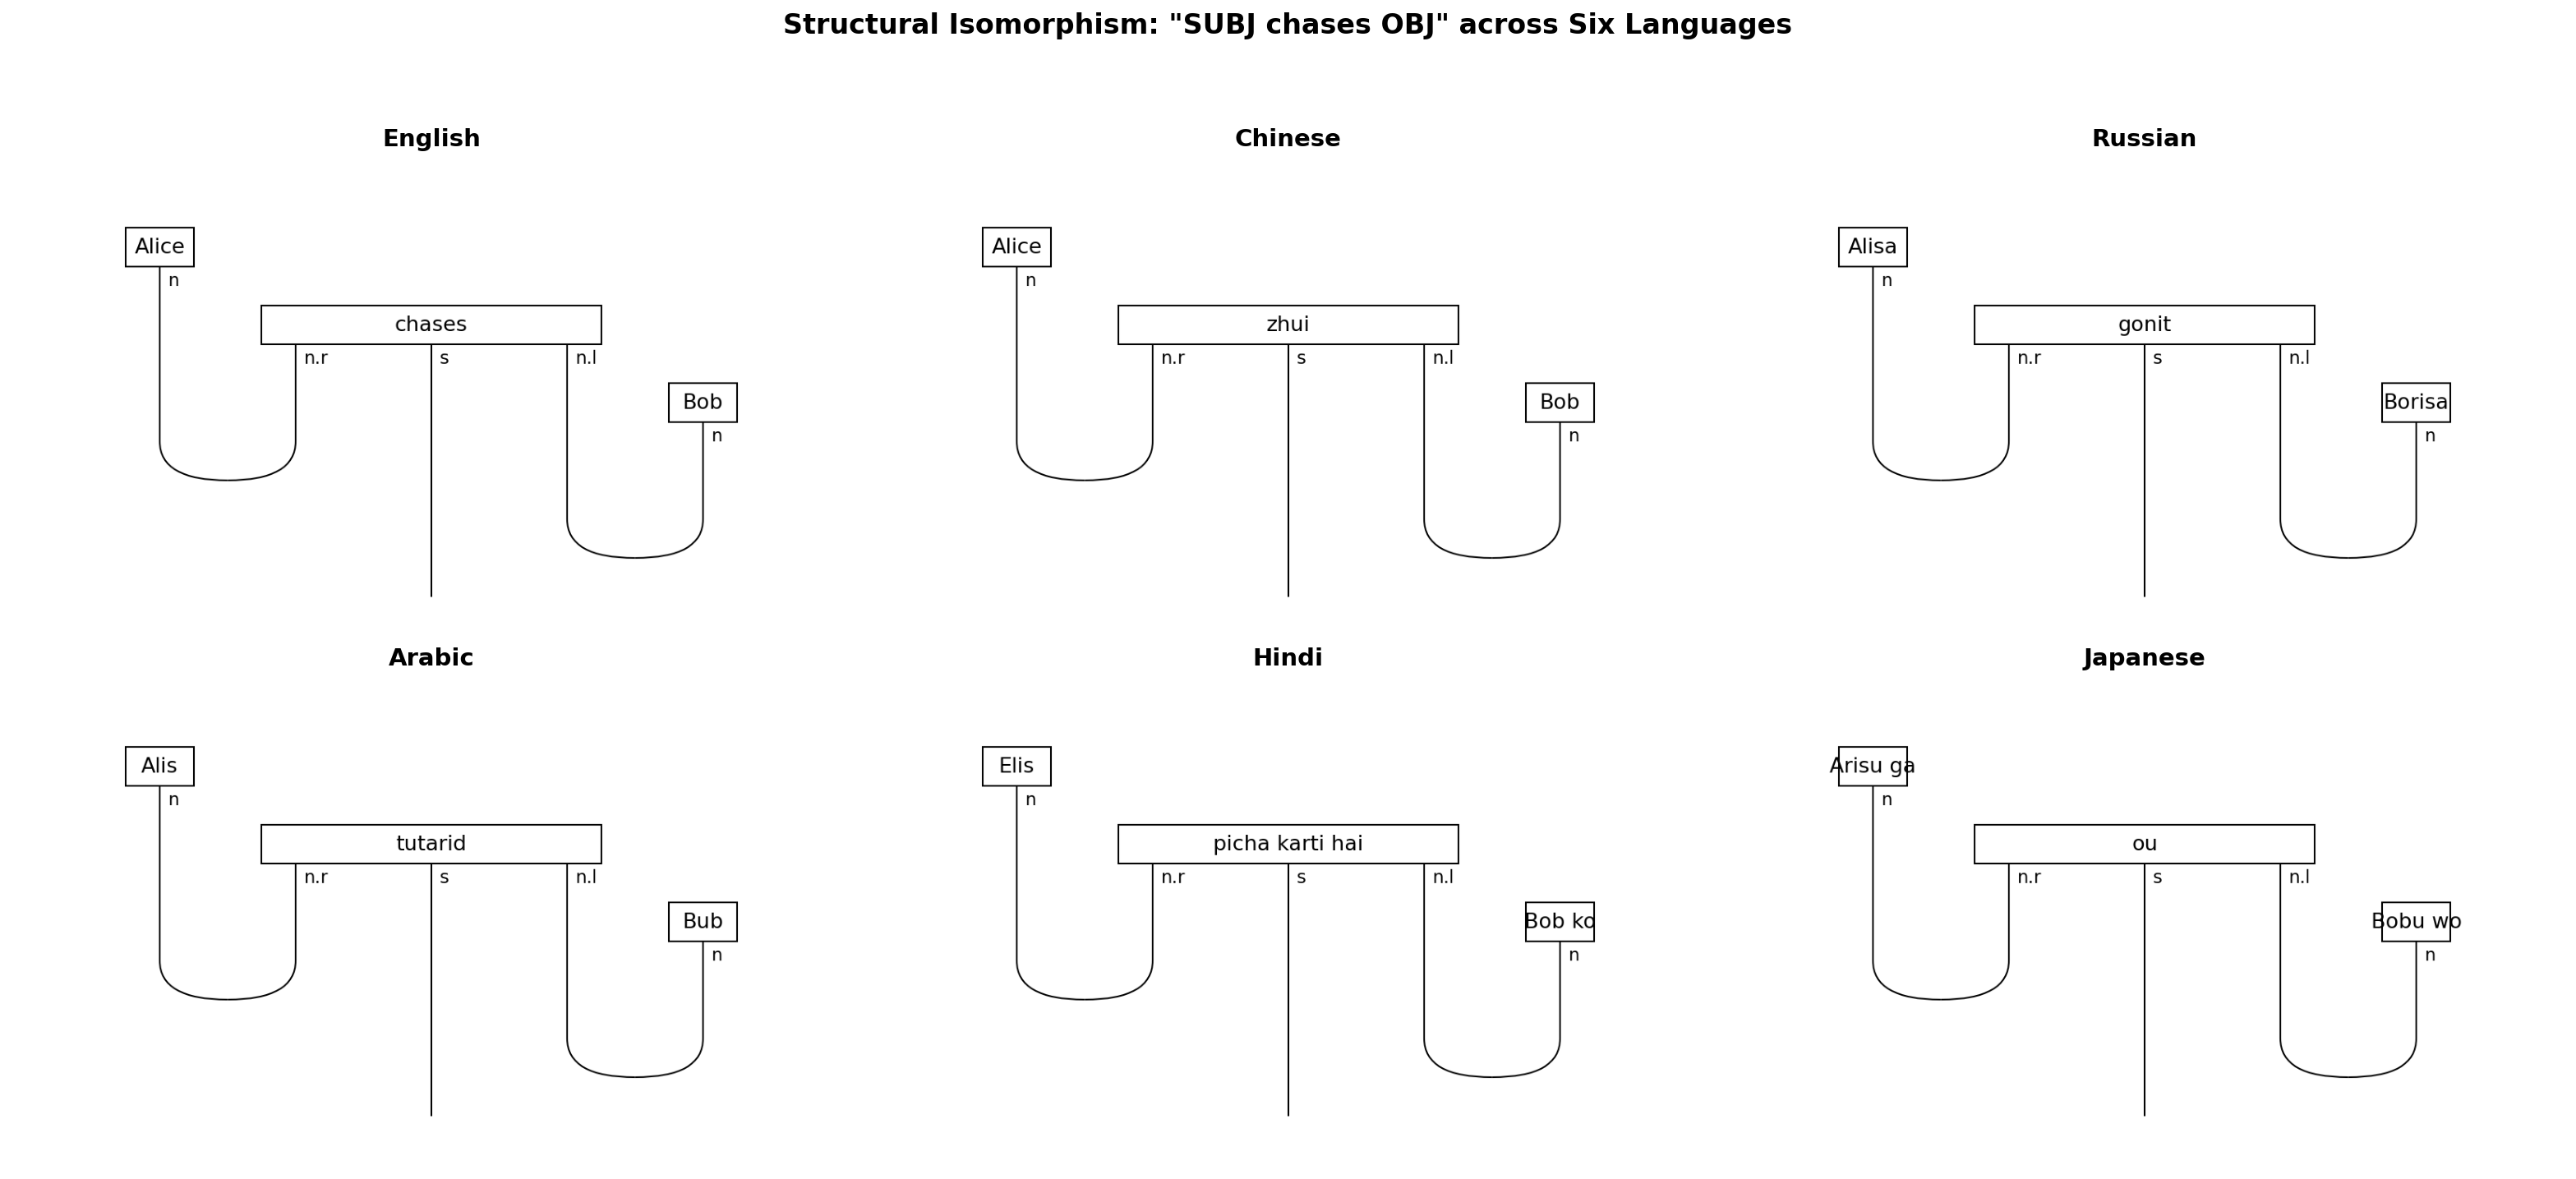
\includegraphics[keepaspectratio,alt={Structural isomorphism of pregroup grammar derivations across six languages: English, Chinese, Russian, Arabic, Hindi, and Japanese. Each panel shows the same transitive sentence (``SUBJ chases OBJ'') rendered as a DisCoPy string diagram with identical type-logical structure --- n ⊗ (n\^{}r ⊗ s ⊗ n\^{}l) ⊗ n → s --- demonstrating that the categorical type reduction is language-invariant despite surface-level morphosyntactic differences.}]{../figures/discopy_multilingual.png}}
\caption{Structural isomorphism of pregroup grammar derivations across
six languages: English, Chinese, Russian, Arabic, Hindi, and Japanese.
Each panel shows the same transitive sentence (``SUBJ chases OBJ'')
rendered as a DisCoPy string diagram with identical type-logical
structure --- n ⊗ (n\^{}r ⊗ s ⊗ n\^{}l) ⊗ n → s --- demonstrating that
the categorical type reduction is language-invariant despite
surface-level morphosyntactic
differences.}\label{fig:multilingual-isomorphism}
\end{figure}

The \emph{soundness and completeness} of string-diagrammatic reasoning
(Joyal--Street theorem) guarantees that any conclusion drawn from the
diagram is algebraically valid.

This visual transparency is precisely the ``free ride'' phenomenon
identified by Shimojima {[}-@shimojima1996reasoning{]}: the diagram
simultaneously represents the syntactic derivation, the argument
structure, and the compositional flow of meaning, without requiring
explicit inference steps to relate them.

\begin{figure}
\centering
\pandocbounded{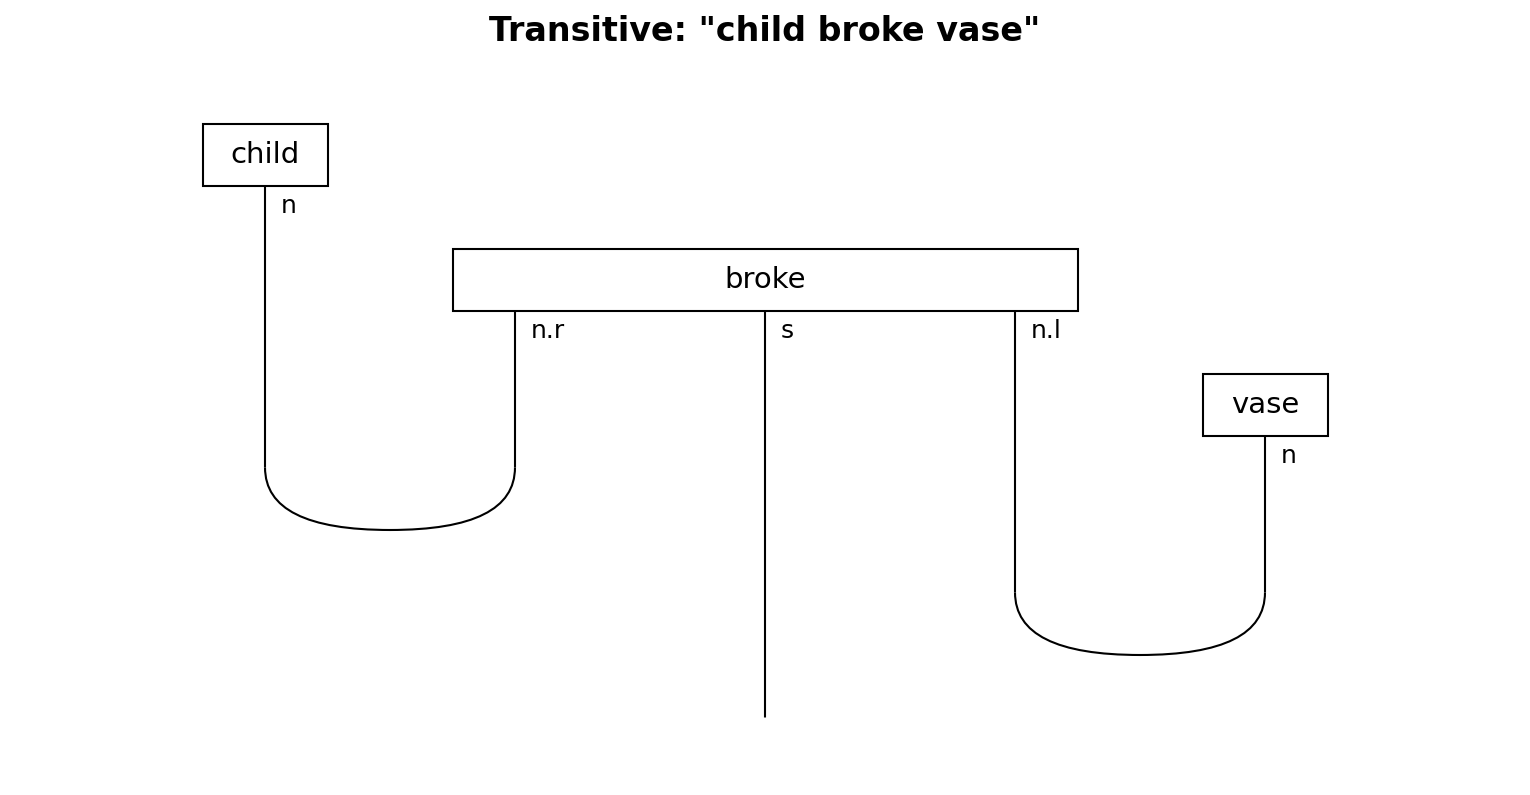
\includegraphics[keepaspectratio,alt={DisCoPy-rendered pregroup grammar diagram for the transitive sentence ``child broke vase,'' produced by the DisCoPy library's native drawing backend. The three Word boxes (child type n, broke type n.r @ s @ n.l, vase type n) are connected by Cup contractions---the leftward cup cancels n with n.r and the rightward cup cancels n.l with n---reducing the entire expression to the sentence type s. The diagrammatic structure makes the type-theoretic derivation immediately inspectable.}]{../figures/discopy_transitive.png}}
\caption{DisCoPy-rendered pregroup grammar diagram for the transitive
sentence ``child broke vase,'' produced by the DisCoPy library's native
drawing backend. The three Word boxes (child type n, broke type n.r @ s
@ n.l, vase type n) are connected by Cup contractions---the leftward cup
cancels n with n.r and the rightward cup cancels n.l with n---reducing
the entire expression to the sentence type s. The diagrammatic structure
makes the type-theoretic derivation immediately
inspectable.}\label{fig:discopy-transitive}
\end{figure}
\end{frame}

\begin{frame}{Case Marking in Type-Logical Categorial Grammar}
\protect\phantomsection\label{case-marking-in-type-logical-categorial-grammar}
Case-marked noun phrases receive compound types that encode both their
grammatical role and their combinatory potential. In a
nominative--accusative language, we can assign:

{\def\LTcaptype{none} % do not increment counter
\begin{longtable}[]{@{}
  >{\raggedright\arraybackslash}p{(\linewidth - 4\tabcolsep) * \real{0.3333}}
  >{\raggedright\arraybackslash}p{(\linewidth - 4\tabcolsep) * \real{0.3333}}
  >{\raggedright\arraybackslash}p{(\linewidth - 4\tabcolsep) * \real{0.3333}}@{}}
\toprule\noalign{}
\begin{minipage}[b]{\linewidth}\raggedright
Expression
\end{minipage} & \begin{minipage}[b]{\linewidth}\raggedright
Type
\end{minipage} & \begin{minipage}[b]{\linewidth}\raggedright
Gloss
\end{minipage} \\
\midrule\noalign{}
\endhead
``Alice'' (subject) & \(n_{\text{NOM}}\) & Noun, nominative-marked \\
``the ball'' (object) & \(n_{\text{ACC}}\) & Noun, accusative-marked \\
``kicks'' & \((n_{\text{NOM}} \backslash s) / n_{\text{ACC}}\) & Seeks
ACC right, NOM left \\
``to Bob'' (recipient) & \((s \backslash s) / n_{\text{DAT}}\) &
Modifies sentence via DAT argument \\
\bottomrule\noalign{}
\end{longtable}
}

The subscripts refine the basic noun type \(n\) with case features,
ensuring that ``kicks'' selects a nominative subject and an accusative
object. Mismatch in case features blocks the derivation, modeling
ungrammaticality.
\end{frame}

\begin{frame}{The Curry--Howard Correspondence and Proof-Theoretic
Semantics}
\protect\phantomsection\label{the-curryhoward-correspondence-and-proof-theoretic-semantics}
A deep structural parallel underlies the Lambek calculus: derivations of
syntactic types correspond to proofs in intuitionistic logic (via the
Curry--Howard isomorphism), and therefore to programs in a typed lambda
calculus. Specifically:

{\def\LTcaptype{none} % do not increment counter
\begin{longtable}[]{@{}
  >{\raggedright\arraybackslash}p{(\linewidth - 4\tabcolsep) * \real{0.3333}}
  >{\raggedright\arraybackslash}p{(\linewidth - 4\tabcolsep) * \real{0.3333}}
  >{\raggedright\arraybackslash}p{(\linewidth - 4\tabcolsep) * \real{0.3333}}@{}}
\toprule\noalign{}
\begin{minipage}[b]{\linewidth}\raggedright
Syntactic Domain
\end{minipage} & \begin{minipage}[b]{\linewidth}\raggedright
Logical Domain
\end{minipage} & \begin{minipage}[b]{\linewidth}\raggedright
Computational Domain
\end{minipage} \\
\midrule\noalign{}
\endhead
Types \((A / B, A \backslash B)\) & Propositions & Types \\
Derivations & Proofs & Programs (\(\lambda\)\text{-terms}) \\
Cut elimination & Proof normalization & \(\beta\)-reduction \\
Commutativity of cuts & Confluence of rewriting & Church--Rosser
property \\
\bottomrule\noalign{}
\end{longtable}
}

This correspondence has two important consequences for our framework:

\begin{enumerate}
\item
  \textbf{Semantic compositionality follows from syntactic
  well-formedness}: a well-typed derivation automatically yields a
  well-formed meaning representation (the \(\lambda\)\text{-term}
  extracted from the proof).
\item
  \textbf{Case assignment is type inference}: determining the case of a
  noun phrase in context is equivalent to inferring the type of a
  variable in a \(\lambda\)\text{-expression}---a computational problem
  with well-understood algorithms.
\end{enumerate}
\end{frame}

\begin{frame}{Monadic Semantics for Sublexical Root Syntax}
\protect\phantomsection\label{monadic-semantics-for-sublexical-root-syntax}
Song {[}-@song2022act; -@song2022blog{]} extends the categorial
framework with a \textbf{monadic semantics} for root syntax, modeling
the sublexical decomposition of verb roots using monads in a syntactic
category. This approach captures the intuition that a verb like
``break'' has internal compositional structure---a causative layer and a
result-state layer---that interacts with case assignment. The monad
encapsulates the complexity of root meaning within a single categorical
construction, allowing the type-logical grammar to handle both lexical
and syntactic composition uniformly.

The monadic approach connects naturally to graded type theory: Asudeh
and Giorgolo {[}-@asudeh2020graded{]} develop a monadic semantics for
evidentiality that uses graded effects to track the epistemic status of
propositions---a pattern that extends to case, where the ``grade'' of a
morphism could encode the strength of a semantic role assignment.
\end{frame}

\begin{frame}[fragile]{Passivization as Algebraic Type Permutation}
\protect\phantomsection\label{passivization-as-algebraic-type-permutation}
One of the most revealing case-theoretic operations is
\textbf{passivization}, which transforms an active transitive clause
into a passive construction by promoting the patient to subject position
and (optionally) demoting the agent to an oblique role. In our
categorical framework, passivization is not an ad hoc syntactic
transformation but a precise \emph{type permutation}---a swap of the
noun types feeding into the verb's pregroup derivation.

In a pregroup grammar, the active transitive ``Alice chases Bob'' has
the type reduction:

\[n_{\text{NOM}} \cdot (n^r \cdot s \cdot n^l) \cdot n_{\text{ACC}} \to s\]

Passivization permutes the noun arguments, yielding ``Bob is chased by
Alice'' with the swapped type assignment:

\[n_{\text{ACC}} \cdot (n^r \cdot s \cdot n^l) \cdot n_{\text{NOM}} \to s\]

Crucially, DisCoPy's \texttt{Swap} primitive makes this permutation
explicit and algebraically precise: the swap operation
\(\sigma_{n,n}: n \otimes n \to n \otimes n\) permutes the two noun
wires without violating the monoidal structure. The resulting diagram
differs from the active version precisely in the crossing of the noun
wires---making the voice alternation \emph{visible} as a topological
feature of the string diagram.

This diagrammatic transparency exemplifies Shimojima's
{[}-@shimojima1996reasoning{]} free-ride inference: by inspecting the
diagram, one can immediately see that passivization preserves the verb's
inherent argument structure while rearranging the surface
realization---a fact that requires multiple inference steps to establish
in a linear notation.

\begin{figure}
\centering
\pandocbounded{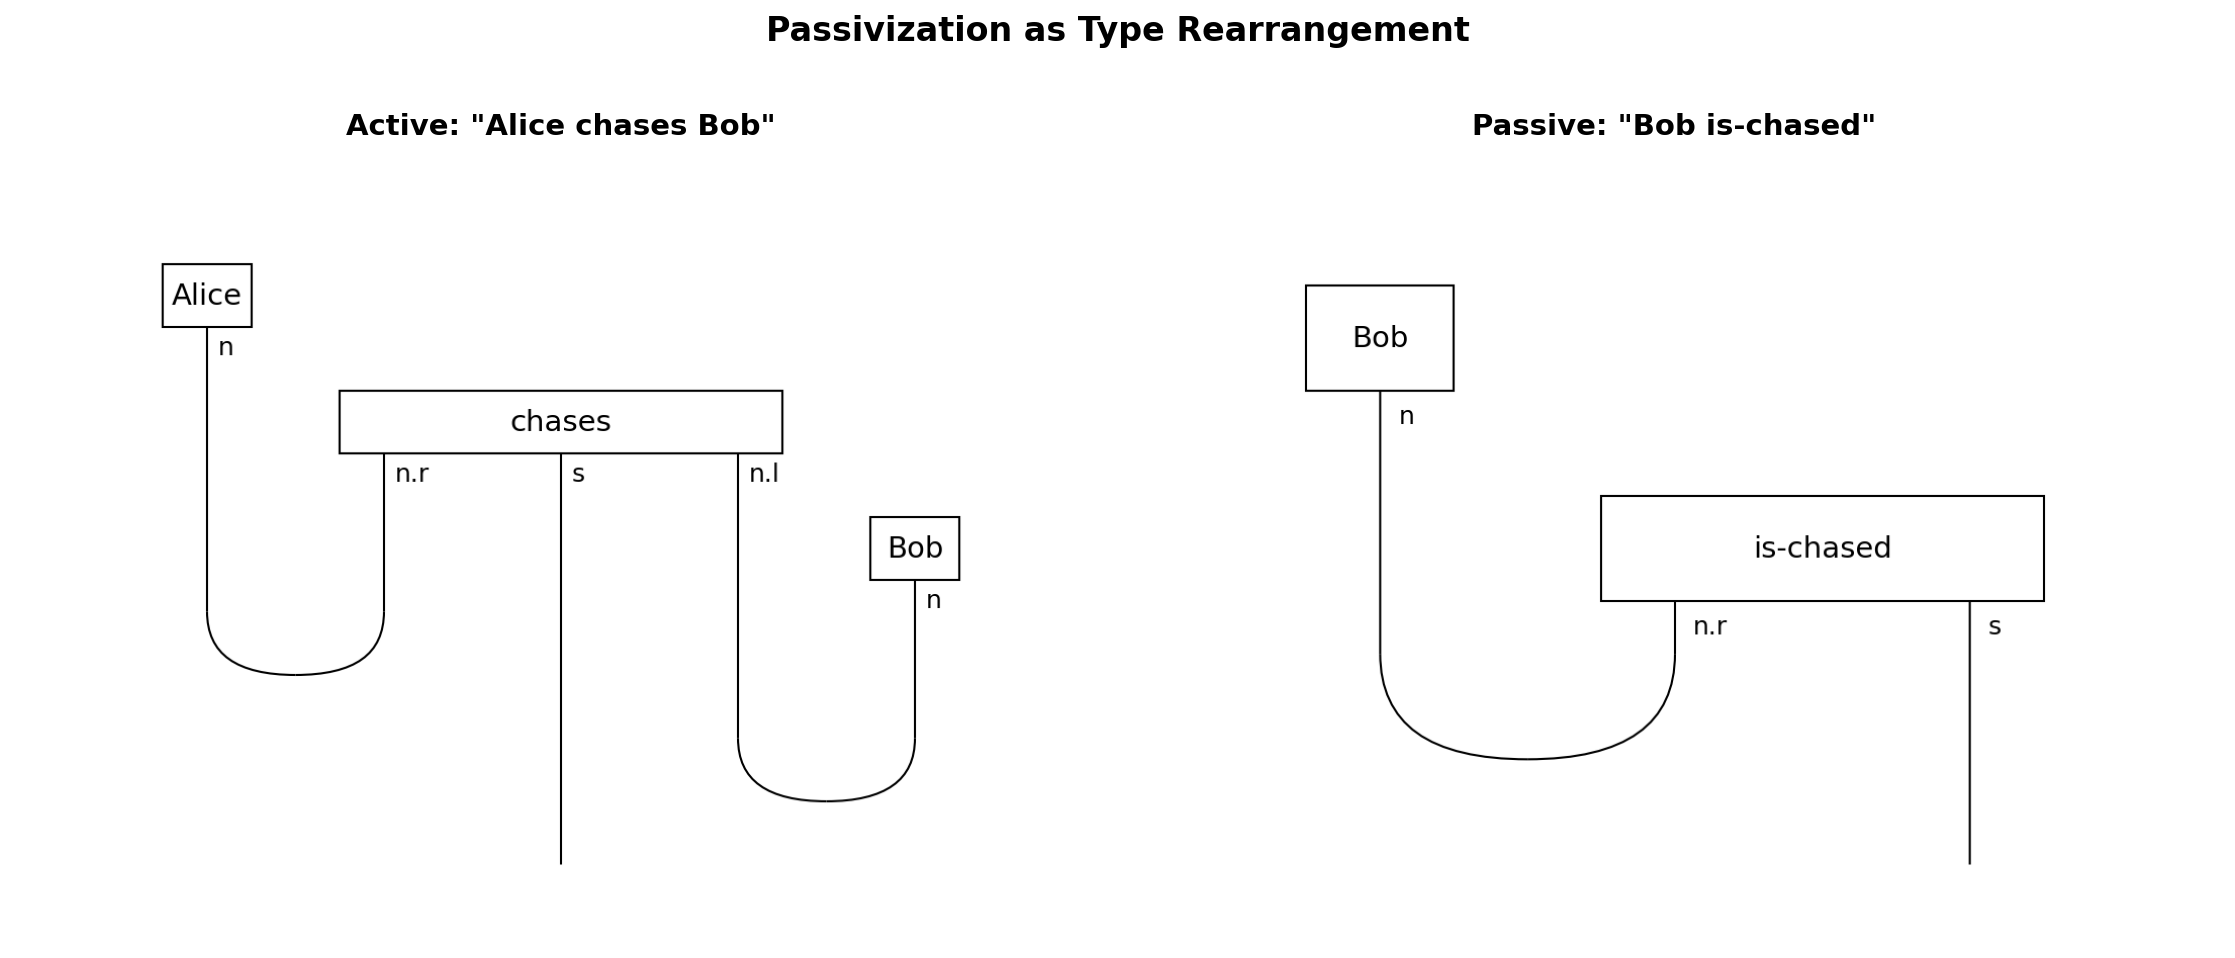
\includegraphics[keepaspectratio,alt={Passivization modeled as a type permutation: the active transitive sentence ``Alice chases Bob'' (left panel) and its passive counterpart ``Bob is-chased'' (right panel), both rendered by DisCoPy. In the active diagram, nom-type Alice feeds the verb's n.r slot while acc-type Bob feeds n.l; in the passive, the patient Bob is promoted to subject (n) position while the verb's type reduces to n.r @ s. The structural difference between voice alternations is visible as a topological change in the wire connectivity.}]{../figures/discopy_passive.png}}
\caption{Passivization modeled as a type permutation: the active
transitive sentence ``Alice chases Bob'' (left panel) and its passive
counterpart ``Bob is-chased'' (right panel), both rendered by DisCoPy.
In the active diagram, nom-type Alice feeds the verb's n.r slot while
acc-type Bob feeds n.l; in the passive, the patient Bob is promoted to
subject (n) position while the verb's type reduces to n.r @ s. The
structural difference between voice alternations is visible as a
topological change in the wire connectivity.}\label{fig:discopy-passive}
\end{figure}
\end{frame}

\end{document}
